\chapter{Eksperymenty obliczeniowe}
\label{ExperimentsChapter}
\vspace*{-1cm}
W tym rozdziale zostanie zaprezentowana część praktyczna tworzonej pracy, która polega na przeprowadzeniu kilku eksperymentów obliczeniowych w oparciu o przygotowane przez autora oprogramowanie. Rozdział rozpoczyna się od omówienia przyjętej metodyki eksperymentów, następnie zostaną przedstawione najistotniejsze szczegóły implementacyjne poszczególnych eksperymentów obliczeniowych. Rozdział zakończy się analizą uzyskanych wyników oraz opisem wypływających z tego wniosków.

\section{Metodyka eksperymentów}
Metodyka eksperymentów obliczeniowych polega na sformułowaniu listy założeń, na których ma się oprzeć przeprowadzenie wszystkich eksperymentów. Oto najważniejsze z przyjętych założeń:
\vspace*{-0.5cm}
\begin{enumerate*}
\item Każdy eksperyment obliczeniowy polega na wytrenowaniu konwolucyjnej sieci neuronowej w przygotowanym Środowisku Uczenia oraz ewaluacji wyuczonego modelu.
\item Parametry dla każdego eksperymentu powinny zostać dostarczone w postaci zewnętrznego pliku konfiguracyjnego o zdefiniowanym formacie. Ścieżkę do pliku konfiguracyjnego należy podać jako argument linii poleceń.
\item Wynikiem przeprowadzonego treningu sieci konwolucyjnej powinien być plik z wytrenowanym modelem.
\item Do samodzielnego przeprowadzenia eksperymentów obliczeniowych należy mieć zainstalowane odpowiednie narzędzia (zgodnie z opisem z rozdziału \ref{DesignSystemChapter}-ciego), jak również posiadać kod źródłowy aplikacji wymaganej do wykonania eksperymentów.
\item Wytrenowany model sieci neuronowej powinien posiadać format danych pozwalający na jego wizualizację przy użyciu zewnętrznego oprogramowania.
\end{enumerate*}

\section{Opis implementacji}
Implementacja systemu została częściowo opisana w rozdziale \ref{ImplementationChapter}-tym, natomiast każdy z przeprowadzonych eksperymentów wymagał dostosowania pewnych detali w implementacji. Poniżej zamieszczam opis tych elementów implementacji, które nie zostały jeszcze opisane, a są zbyt ważne aby je pominąć.

\subsection{Środowiska Uczenia}
\label{LearningEnvsSubsection}
W ramach prac nad częścią eksperymentalną zostały przygotowane 3 Środowiska Uczenia, będące niczym innym jak scenami silnika Unity. Każde Środowisko Uczenia posiada własną charakterystykę oraz pewne cechy szczególne, wyróżniające je na tle pozostałych Środowisk.

\subsubsection{RaceTrack\_1}
Te Środowisko Uczenia zostało oparte na torze wyścigowym ,,\textit{Figure 8 Track}'' z pakietu \textbf{Environmental Race Track Pack} (por. \ref{RaceTracksSection}). Najważniejszą cechą Środowiska jest brak oświetlenia, co zostało dołożone w kolejnych Środowiskach. Wykorzystaną tutaj implementacją klasy Agent jest \textit{SimpleCarAgent} (por. \ref{AgentImplementations}). Rysunek \ref{RaceTrack1AgentComps} przedstawia najważniejsze komponenty obiektu sceny \textit{CarAgent}. \\
\begin{figure}[h]
\begin{center}
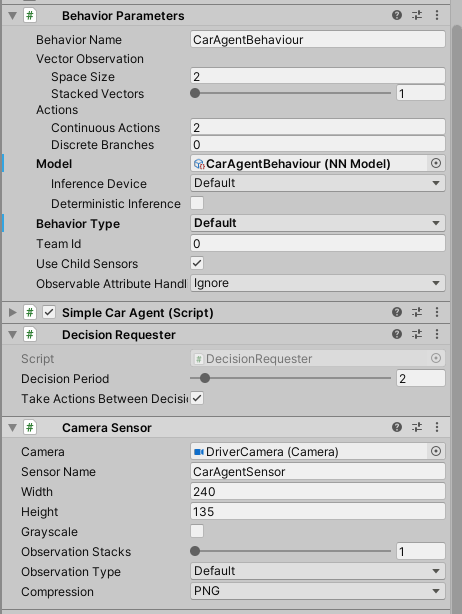
\includegraphics[width=9cm]{resources/figures/race_track_1_agent_components.png}
\caption{Najważniejsze komponenty obiektu \textit{CarAgent} w Środowisku Uczenia \textit{RaceTrack\_1}}
\label{RaceTrack1AgentComps}
\end{center}
\end{figure}
\noindent
Na podstawie rysunku można wysnuć kilka wniosków:
\vspace{-0.5cm}
\begin{itemize*}
\item Do agenta są dostarczane dwie obserwacje wektorowe;
\item Agent jest zobligowany do wykonywania dwóch akcji dla każdego kroku symulacji;
\item Wykorzystaną implementacją klasy \textit{Agent} jest klasa \textit{SimpleCarAgent};
\item Decyzje są podejmowane dla co drugiego kroku symulacji. Pomiędzy decyzjami należy wykonywać ostatnio obliczone Akcje;
\item Wykorzystywane są obserwacje wizualne w postaci pojedynczego czujnika, zbierającego obraz z kamery umieszczonej na miejscu fotela kierowcy. Obserwacje wizualne mają rozdzielczość $240 \times 135$ pikseli. Rysunek \ref{RaceTrack1Cockpit} przedstawia widok z kamery stanowiącej źródło danych wejściowych dla obserwacji wizualnych.
\end{itemize*}

\begin{figure}[h]
\begin{center}
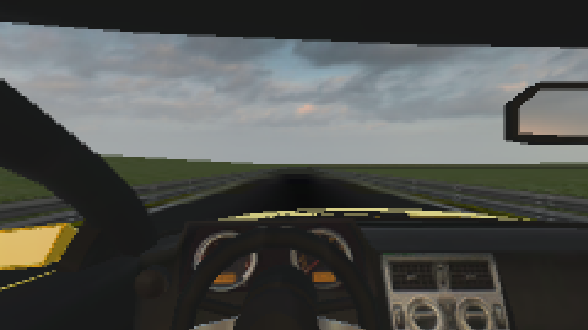
\includegraphics[width=15cm]{resources/figures/race_track_1_cockpit.png}
\caption{Widok z fotela kierowcy w Środowisku Uczenia \textit{RaceTrack\_1}}
\label{RaceTrack1Cockpit}
\end{center}
\end{figure}

\subsubsection{RaceTrack\_2}
Jest to Środowisko \textit{RaceTrack\_1} z dodanym oświetleniem, którego parametry są losowo ustawiane przed rozpoczęciem każdego epizodu symulacji. Parametry oświetlenia ulegające zmianie to \textbf{pozycja}, \textbf{rotacja} (orientacja), \textbf{kolor} oraz \textbf{intensywność}.

\subsubsection{RaceTrack\_3}
Środowisko Uczenia oparte na torze wyścigowym ,,,\textit{Coastal Race Track}'' z pakietu \textbf{Environmental Race Track Pack} (por. \ref{RaceTracksSection}). Ponieważ tor wyścigowy jest bardziej skomplikowany, przygotowana została nowa implementacja klasy \textit{Agent} - klasa \textit{AdvancedCarAgent}. Reszta komponentów obiektu sceny \textit{CarAgent} pozostała bez zmian. Rysunek \ref{RaceTrack3Cockpit} przedstawia widok z kamery dla tego Środowiska Uczenia. \\

\begin{figure}[h]
\begin{center}
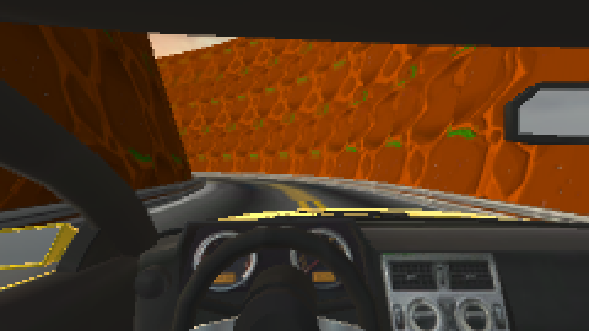
\includegraphics[width=15cm]{resources/figures/race_track_3_cockpit.png}
\caption{Widok z fotela kierowcy w Środowisku Uczenia \textit{RaceTrack\_3}}
\label{RaceTrack3Cockpit}
\end{center}
\end{figure}

\subsection{Implementacje klasy Agent}
\label{AgentImplementations}
W toku prac nad aplikacją zostało napisanych i przetestowanych wiele wersji implementacji klasy \textit{Agent} z zestawu Unity ML-Agents, jednak ostatecznie do wykorzystania zostały wyznaczone dwie klasy: \textit{SimpleCarAgent} oraz \textit{AdvancedCarAgent}. Chociaż są do siebie podobne, to jednak istnieje kilka różnic na które koniecznie trzeba zwrócić uwagę.

\subsubsection{SimpleCarAgent}
Klasa użyta w Środowiskach Uczenia \textit{RaceTrack\_1} oraz \textit{RaceTrack\_2} (por. \ref{LearningEnvsSubsection}). Jest odpowiedzialna za:
\vspace*{-0.5cm}
\begin{enumerate*}
\item \textit{Prawidłową inicjalizację każdego epizodu treningu} - przywrócenie samochodu do pozycji startowej oraz zmianę właściwości oświetlenia (jego pozycji, orientacji, koloru oraz intensywności).
\item \textit{Przekazywanie obserwacji ze Środowiska Uczenia do sieci neuronowej} - pobierane są 3 obserwacje ze środowiska - jedna wizualna (obraz z kamery) oraz dwie wektorowe (znormalizowana prędkość samochodu oraz informacja o tym, czy w danej chwili samochód dotyka jakiejś przeszkody).
\item \textit{Przekazywanie wyjścia z sieci neuronowej do Środowiska Uczenia} - sieć neuronowa generuje dwie wartości (zwane Akcjami), które są liczbami rzeczywistymi z domkniętego przedziału od $-1$ do $1$. Pierwsza wartość to stopień wciśnięcia pedału hamulca lub przepustnicy (gdzie $-1$ to maksymalnie wciśnięty hamulec, a $1$ to maksymalnie wciśnięta przepustnica), a druga to kąt skrętu kierownicy (gdzie $0$ oznacza jazdę na wprost, $-1$ maksymalny skręt w lewo a $1$ maksymalny skręt w prawo).
\item \textit{Obliczanie wartości sygnałów nagrody dla danego kroku symulacji} - sygnały nagród są obliczane na podstawie dwóch przesłanek: prędkości samochodu oraz kolizji z przeszkodami. Nagroda za prędkość jest proporcjonalna do prędkości samochodu, co oznacza że większa prędkość oznacza większą nagrodę. Za kolizje z przeszkodami przyznawane są kary, proporcjonalne do prędkości z jaką doszło do kolizji z przeszkodą. Dodatkowo przyznawana jest kara o stałej wartości za każdy krok symulacji, w którym samochód styka się z jakąś przeszkodą.
\end{enumerate*}
\noindent
Zmienne publiczne, jakie można przypisać do tej klasy z poziomu edytora Unity, to:
\vspace*{-0.5cm}
\begin{itemize*}
\item \texttt{MaxStep} - maksymalna liczba kroków symulacji dla danego epizodu;
\item \texttt{CarAgentObject} - Referencja na obiekt sceny \textit{CarAgent};
\item \texttt{StartCarPosition} - Pozycja początkowa samochodu;
\item \texttt{StartCarRotation} - Orientacja początkowa samochodu;
\item \texttt{DirectionalLight} - Referencja na obiekt oświetlenia (może być pusta, jeśli oświetlenie nie jest używane).
\end{itemize*}

\subsubsection{AdvancedCarAgent}
Klasa użyta w Środowisku Uczenia \textit{RaceTrack\_3} (por. \ref{LearningEnvsSubsection}). Posiada dokładnie te same odpowiedzialności co klasa \textit{SimpleCarAgent}, jak również większość kodu jest taka sama. Główna różnica polega na tym, że klasa \textit{AdvancedCarAgent} wspiera możliwość resetowania samochodu przy starcie nowego epizodu do wielu różnych pozycji oraz orientacji. Listę pozycji i orientacji można uzupełniać z poziomu edytora Unity, co widać na rysunku \ref{AdvancedCarAgentLocList}, gdzie został zaprezentowany fragment listy \texttt{StartCarLocations}. \\

\begin{figure}[h]
\begin{center}
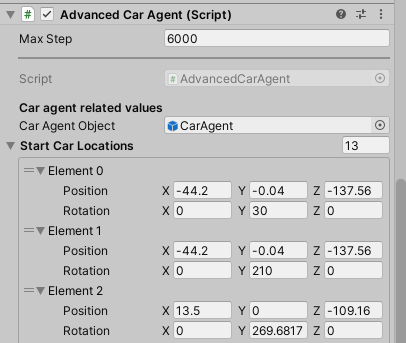
\includegraphics[width=6.5cm]{resources/figures/advanced_car_agent_loc_list.png}
\caption{\textit{AdvancedCarAgent} - fragment listy \texttt{StartCarLocations}.}
\label{AdvancedCarAgentLocList}
\end{center}
\end{figure}

\subsection{Konfiguracja treningu}
Konfiguracja treningu odbywa się poprzez przygotowanie pliku konfiguracyjnego w formacie YAML \cite{unitymla:configFile}. Dla każdego Środowiska Uczenia został przygotowany osobny plik konfiguracyjny, jednak różnice pomiędzy nimi są kosmetyczne i dotyczą detali. Oto zawartość pliku konfiguracyjnego dla Środowiska \textit{RaceTrack\_3}:

\begin{minted}[ fontsize=\fontsize{10}{9} ] {yaml}
engine_settings:
  width: 240
  height: 135
  quality_level: 5
  time_scale: 20
  target_frame_rate: -1
  capture_frame_rate: 60
  no_graphics: false
torch_settings:
  device: cuda
behaviors:
  CarAgentBehaviour:
    trainer_type: ppo
    summary_freq: 50000
    time_horizon: 256
    max_steps: 30000000
    keep_checkpoints: 10
    checkpoint_interval: 500000
    threaded: true
    network_settings:
      hidden_units: 128
      num_layers: 2
      normalize: true
      vis_encode_type: simple
      conditioning_type: none
    reward_signals:
      extrinsic:
        strength: 1.0
        gamma: 0.99
\end{minted}

Najważniejsze ustawienia dotyczą sekcji \texttt{behaviors}, ponieważ one mają największy wpływ na kształt treningu. W tym miejscu warto omówić kilka z nich:
\begin{enumerate*}
\item \texttt{trainer\_type} - wybór algorytmu uczącego. Dla wszystkich eksperymentów obliczeniowych wybrano algorytm PPO \cite{ppo:opis}, ponieważ w toku prac nad aplikacją okazał się być lepszym wyborem niż SAC \cite{sac:opis};
\item \texttt{time\_horizon} - jak wiele kroków symulacji należy zebrać przed dodaniem ich do ,,bufora doświadczenia''. Wartość parametru powinna znajdować się w kompromisie pomiędzy mniej stronniczym, ale wyższym oszacowaniem wariancji (długi horyzont czasowy) i bardziej stronniczym, ale mniej zróżnicowanym oszacowaniem (krótki horyzont czasowy). Gdy nagrody są często przyznawane lub epizody trwają dość długo, wtedy mniejsza liczba może być lepszym wyborem. Niemniej jednak, wartość ta powinna być na tyle duża, aby można było uchwycić wszystkie ważne zachowania w sekwencji działań agenta;
\item \texttt{max\_steps} - maksymalna liczba kroków symulacji przed zakończeniem treningu;
\item \texttt{keep\_checkpoints} - maksymalna liczba modeli sieci neuronowych, pozostawionych do zapisu. Modele te są zapisywane w odstępach określonych wartością parametru \texttt{checkpoint\_interval}, która oznacza interwał czasowy wyrażony w krokach symulacji treningowej; 
\item \texttt{network\_settings} - ustawienia sieci neuronowej. Najważniejsze z nich to:
\begin{itemize*}
\item \texttt{hidden\_units} - liczba neuronów w pełni połączonej warstwie ukrytej;
\item \texttt{num\_layers} - liczba warstw ukrytych;
\item \texttt{vis\_encode\_type} - typ enkodera dla obserwacji wizualnych.
\end{itemize*}
\end{enumerate*}

Rozpoczęcie treningu sieci odbywa się poprzez wywołanie komendy \texttt{mlagents\_learn}, której dokładne wykorzystanie zostało opisane w dokumentacji zestawu Unity ML-Agents \cite{unitymla:trainingMlAgents}.

\section{Przebieg eksperymentów i analiza wyników}
Dla każdego z przygotowanych Środowisk Uczenia przeprowadzono dokładnie jeden eksperyment obliczeniowy, polegający na wytrenowaniu konwolucyjnej sieci neuronowej do jazdy samochodem po wybranym torze wyścigowym, a następnie ewaluacji wytrenowanego modelu pod kątem przystosowania do rzeczywistej funkcji celu, jaką jest pokonanie toru wyścigowego w możliwie najkrótszym czasie.

\subsection{RaceTrack\_1}
Środowisko najłatwiejsze do wytrenowania konwolucyjnej sieci neuronowej, ponieważ brak jest zmiennego oświetlenia sceny, a zakręty są łagodne i niewymagające trudnych manewrów do wykonania. Wytrenowanie modelu zajęło 1647798 kroków symulacji. \\
Obserwacje sieci obejmowały:
\vspace*{-0.5cm}
\begin{enumerate*}
\item Obserwacje wizualne z kamery umieszczonej na fotelu kierowcy, czyli obrazki RGB o wymiarach $240 \times 135$ pikseli;
\item Obserwacje wektorowe:
\begin{itemize*}
\item Bieżąca, znormalizowana prędkość samochodu;
\item Wartość logiczna informująca, czy samochód w danej chwili styka się z jakąś przeszkodą.
\end{itemize*}
\end{enumerate*}

Model był trenowany na pojedynczej instancji obiektu sceny \textit{CarAgent}, którego pozycja i orientacja były resetowane na początku każdego epizodu symulacji. Epizod kończył się w momencie przejechania pełnego okrążenia lub po wyczerpaniu zakładanego limitu czasowego dla danego epizodu. Z obserwacji wytrenowanego modelu wynika, że:
\vspace*{-0.5cm}
\begin{enumerate*}
\item Model charakteryzuje się niestabilnym tempem jazdy, a wykonane pomiary czasowe wskazują na dość znaczne odchyły w czasach okrążeń.
\item Wytrenowany model jest w stanie bezpiecznie przejechać kilka okrążeń pod rząd, choć ma tendencje do bardzo agresywnego wchodzenia w pierwszy zakręt, co czasem kończy się poważną kraksą - samochód obraca się o 90 stopni w stosunku do zakładanego kierunku jazdy.
\item Po wystąpieniu poważnej kraksy, wytrenowany model nie potrafi zazwyczaj wrócić do dalszej jazdy, lecz stara się zminimalizować straty poprzez oddalenie się od barierki, tak aby nie było naliczanej kary za kontakt z przeszkodami.
\item Model radzi sobie z jazdą tylko wtedy, gdy kolor drogi wyraźnie kontrastuje z poboczem - przy załączonym oświetleniu kierunkowym sieć się gubi, dojeżdżając do miejsca gdzie droga zbyt się rozjaśnia z powodu oświetlenia.
\end{enumerate*}

\subsection{RaceTrack\_2}
Środowisko Uczenia bardzo podobnie skonfigurowane do \textit{RaceTrack\_1}, jednak z jedną zasadniczą różnicą - trening odbywał się przy załączonym oświetleniu kierunkowym, którego właściwości były losowo ustawiane dla każdego epizodu treningowego. Model został wytrenowany po 4654498 krokach symulacji. Obserwacje modelu wykazały, że:
\begin{enumerate*}
\item Jego tempo jazdy jest znacznie stabilniejsze od poprzedniego modelu, ponieważ różnice między najszybszym i najwolniejszym okrążeniem były średnio 4-krotnie mniejsze niż dla poprzedniego modelu.
\item Model wciąż wykazuje tendencje do agresywnego wchodzenia w pierwszy zakręt, co często kończy się poważną kraksą.
\item Po wystąpieniu poważnej kraksy (obrócenie o 90 stopni lub więcej), samochód staje w miejscu lub wręcz zawraca i zaczyna jechać ,,pod prąd''. Pod tym względem zachowanie tego modelu niezbyt odbiega od zachowania modelu poprzedniego.
\item Model dobrze sobie radzi ze zmiennym oświetleniem, chociaż wciąż się gubi dla niektórych przypadków brzegowych.
\end{enumerate*}

\subsection{RaceTrack\_3}
W tym Środowisku Uczenia trening potrwał znacznie dłużej niż na obydwu poprzednich Środowiskach razem wziętych i wyniósł prawie 13 milionów kroków symulacji (było to dokładnie 12999786). Wynika to z faktu, że te Środowisko jest dużo trudniejsze do wytrenowania, ponieważ tor wyścigowy jest bardziej zróżnicowany i składa się z zakrętów o bardziej odmiennej charakterystyce. Z obserwacji wytrenowanego modelu wynika, że:
\begin{enumerate*}
\item Jego zachowanie jest dosyć nierówne. Z jednej strony, zdarza się że przez dłuższy odcinek czasu samochód całkiem znośnie pokonuje kolejne zakręty, zwalniając przed ostrzejszymi nawrotami. Z drugiej strony, chwilę później na łagodniejszym zakręcie samochód potrafi uderzyć pełnym impetem w barierkę, obrócić się bokiem do drogi i dalej nie ruszyć.
\item Model wypracował sobie strategię utrzymania toru jazdy samochodu przy mocnym zderzeniu z barierką na ostrym zakręcie. W takich sytuacjach następuje skręt kierownicy do skrajnej pozycji w kierunku zakrętu - czyli przy zakręcie w lewo następuje maksymalny skręt kierownicą na lewo.
\item Jeśli samochód po kraksie nie jest obrócony prostopadle do kierunku jazdy, lecz pod pewnym mniejszym kątem, to wtedy jest szansa że samochód powróci do dalszej jazdy. Jeśli jednak samochód obróci się o więcej niż 90 stopni, to nie zawróci, ponieważ model nie posiada żadnych informacji na temat tego, w którą stronę samochód powinien się poruszać. W najlepszym wypadku samochód ruszy w drugą stronę.
\item Podobnie jak poprzedni model, całkiem dobrze radzi sobie ze zmiennym oświetleniem.
\item Przejeżdżając przez ciasne nawroty, samochód zwalnia aby uniknąć kolizji. W skrajnych przypadkach potrafi całkowicie się zatrzymać i dalej nie ruszyć, pomimo tego że sytuacja pozwalałaby na dalszą jazdę.
\end{enumerate*}

\section{Analiza wytrenowanego modelu}
Model wytrenowany w Środowisku \textit{RaceTrack\_3} został załadowany do programu o nazwie Netron (por. \ref{NetronOpis}). Rysunek \ref{ModelVisualization} przedstawia wizualizację załadowanego modelu. \\

\begin{figure}[h]
\begin{center}
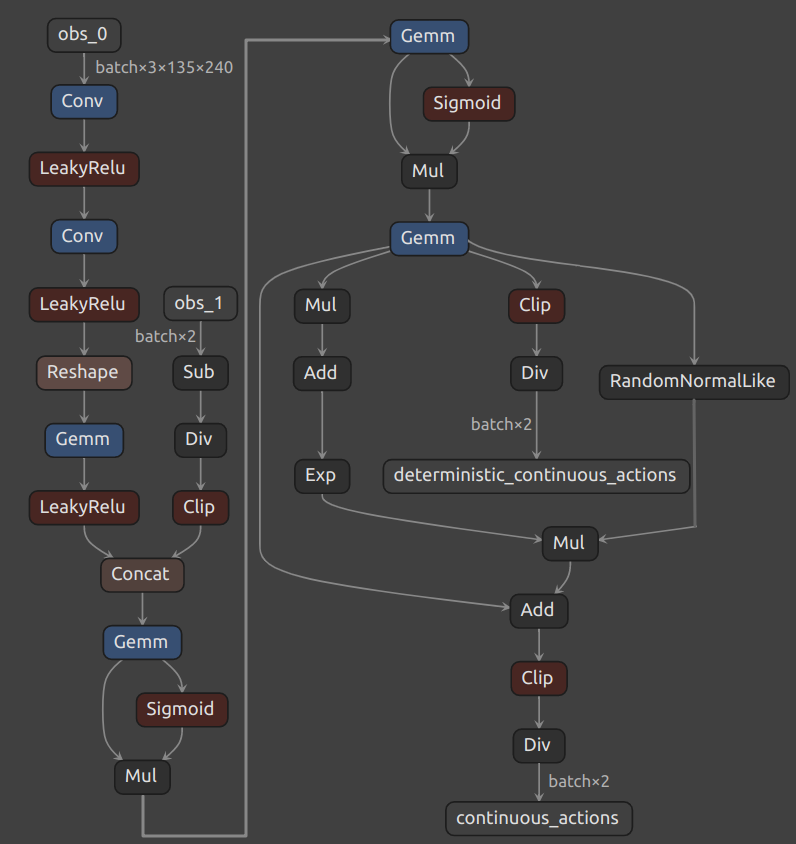
\includegraphics[width=13.5cm]{resources/figures/model_visualization.png}
\caption{Wizualizacja modelu wytrenowanego w Środowisku Uczenia \textit{RaceTrack\_3}}
\label{ModelVisualization}
\end{center}
\end{figure}

\begin{figure}[h]
\begin{center}
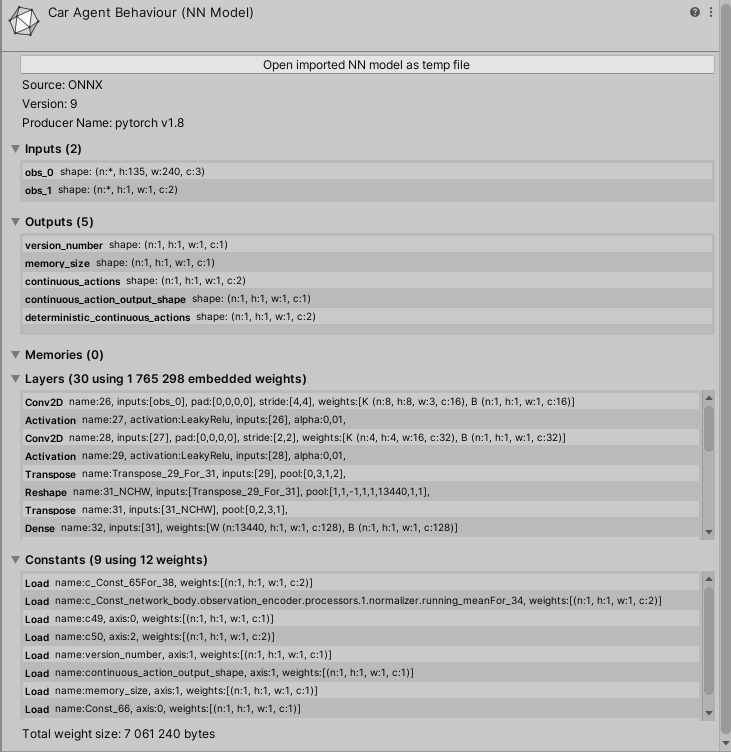
\includegraphics[width=13.5cm]{resources/figures/trained_model_inspector.png}
\caption{Podgląd wytrenowanego modelu w inspektorze edytora Unity}
\label{TrainedModelInspector}
\end{center}
\vspace*{-0.5cm}
\end{figure}

Więcej informacji na temat każdego z operatorów (czyli typów warstw sieci) można znaleźć na stronie dokumentacji standardu ONNX \cite{onnx:operators}. Wykorzystane operatory posiadają następujące znaczenie:
\vspace*{-0.5cm}
\begin{enumerate*}
\item \textbf{obs\_0}, \textbf{obs\_1} - obserwacje wejściowe (odpowiednio: wizualne i wektorowe);
\item \textbf{Conv} - warstwa konwolucyjna;
\item \textbf{LeakyRelu} - funkcja aktywacji LeakyRelu;
\item \textbf{Reshape} - warstwa zmieniająca kształt (wymiary) danych wejściowych;
\item \textbf{Add}, \textbf{Sub}, \textbf{Mul}, \textbf{Div} - operacje dodawania, odejmowania, mnożenia i dzielenia;
\item \textbf{Clip} - operacja obcinania wartości do zadanej dziedziny;
\item \textbf{Concat} - warstwa łącząca;
\item \textbf{Gemm} - warstwa ogólnego mnożenia macierzy;
\item \textbf{Sigmoid} - funkcja aktywacji Sigmoid;
\item \textbf{Exp} - operacja potęgowania;
\item \textbf{RandomNormalLike} - generator tensorów losowych.
\end{enumerate*}

Ten sam model można również podejrzeć w inspektorze edytora Unity, co zostało zaprezentowane na rysunku \ref{TrainedModelInspector}. Wytrenowany model składa się z 30 warstw oraz 1765298 wag, których wartości musiały być dostrojone podczas trwania treningu. Cały plik modelu ma rozmiar 7061240 bajtów, co w przybliżeniu daje nam 6,73 MB.

W tym miejscu należy wyjaśnić, dlaczego zastosowano powyżej opisaną architekturę modelu sieci. Powody są następujące:
\begin{enumerate*}
\item Punktem wyjścia była chęć przeprowadzenia treningu w oparciu o dane wizualne, a do takich zadań doskonałym wyborem są konwolucyjne sieci neuronowe (por. rozdział \ref{CNNsChapter}-gi). Dlatego architektura sieci posiada warstwy konwolucyjne.
\item Dwie warstwy konwolucyjne są domyślnym wyborem, oferowanym przez zestaw Unity ML-Agents. Po  kilku testach, autor postanowił pozostać przy tej wartości, ponieważ okazała się być wystarczająco dobra dla potrzeb treningu.
\item Autor eksperymentował z różnymi rozdzielczościami obrazu wejściowego, rozpoczynając od możliwie najmniejszych wartości. Taki kierunek poszukiwań wydawał się właściwy, ponieważ mniejsze dane wejściowe oznaczają zwykle krótszy trening, a w konsekwencji szybszą ewaluację zaprojektowanego modelu. Jednakże zbyt niska rozdzielczość to brak detali istotnych do nauczenia się modelu, dlatego wybór właściwej rozdzielczości jest zawsze kwestią kompromisu. Po wielu testach, autor ostatecznie przyjął rozdzielczość $240 \times 135$, ponieważ przy niższej rozdzielczości ciasne nawroty były zauważane zbyt późno i model nie miał możliwości dohamować przed zakrętem.
\item Pozostałe elementy architektury sieci pochodzą z domyślnej konfiguracji zestawu Unity ML-Agent. Konfiguracja ta okazała się sprawdzać bardzo dobrze, dlatego autor pracy postanowił przy niej pozostać.
\end{enumerate*}

\section{Wnioski}
W wyniku przeprowadzonych eksperymentów obliczeniowych, autor niniejszej pracy sformułował kilka wniosków:

\begin{enumerate*}
\item Złożoność Środowiska Uczenia w bezpośredni sposób przekłada się na długość treningu sieci neuronowej. Pomimo braku zmian w topologii sieci, jej hiperparametrach czy też algorytmie uczącym, każde kolejne z opisanych Środowisk Uczenia wymagało zauważalnie więcej obliczeń podczas treningu modelu. Wynikało to z faktu, że każde kolejne Środowisko było bardziej różnorodne, co utrudniało algorytmowi uczącemu odnalezienie powiązań między wzorcami wizualnymi i oczekiwanymi akcjami.
\item Zaprojektowana funkcja nagród (zależna od prędkości samochodu oraz występujących kolizji) okazała się być wystarczająca jedynie dla wyuczenia się podstawowych manewrów, takich jak jazda po prostej oraz bezkolizyjne pokonywanie łagodnych zakrętów. Przejeżdżając przez ciaśniejsze zakręty, model wykazuje zbyt agresywne zachowanie, co zazwyczaj kończy się poważną stłuczką i brakiem możliwości dalszej jazdy. Aby to zmienić, funkcję nagród należałoby przeprojektować, co jest zadaniem wysoce nietrywialnym i wymagającym wiele czasu poświęconego na testowanie różnych rozwiązań.
\item Pomimo treningu przy zmiennym oświetleniu, rodzaj i natężenie oświetlenia wciąż mają istotny wpływ na jakość zachowania modelu.
\item Model wytrenowany na jednym Środowisku Uczenia nie potrafi się poprawnie zachować na pozostałych Środowiskach. Powodów takiego stanu rzeczy należałoby upatrywać w zauważalnych różnicach wizualnych pomiędzy Środowiskami.
\item Uzyskane wyniki eksperymentów pozwalają na zaobserwowanie korelacji pomiędzy Środowiskiem Uczenia a długością treningu, natomiast nie wnoszą żadnej wiedzy na temat wpływu konfiguracji na skuteczność wyuczonego modelu. Dalsze badania w tym zakresie są jak najbardziej wskazane.
\end{enumerate*}